\documentclass[./main.tex]{subfiles}

\begin{document}

\chapter{Introduction}\label{chapter:introduction}

"Only what is evolving is alive" \footnote{Pierre Kerner translation from french, original quote "N'est vivant que ce qui évolue"} this definition of life, like many others, is incomplete and we can probably find some corner case. This definition is based on the definition of evolution. We can try to define the evolution of a thing as the change on the thing to optimize its capability to conserve itself. To do that a thing need a memory.

In the majority of current know life, the physical support of this memory was DNA for DeoxyriboNucleic Acid. DNA is a molecule composed of two strains. Each strain is composed of a phosphate backbone. Along these backbones, we have a sugar linked to a nucleic acid. We have four types of nucleic acid: Adenine (A), Thymine (T), Cytosine (C) and Guanine (G), Figure \ref{intro:fig:dna_rna_pres} shows the 3d structure of DNA.

The two strands of DNA are linked by their nucleic acids, with some rules. In front of an, A we will always have a T, in front of a C we will always have a G and vice versa. A DNA strain is a complementary of the other. But we cannot add a new DNA base to each DNA strain at the same end, for some of chemical properties that we will not detail here. We say DNA is composed of two anti-parallel strains. By convention we always represent DNA in the same orientation.

In bioinformatics, we generally represent a DNA strain by a string an a four letter alphabet (A, C, T, G). The two property describe earlier allow us to reconstruct the composition of one strand from the other by  complementary (replace A by T, T by A, C by G and G by C) and reverse order.

\begin{figure}[ht]
    \centering
    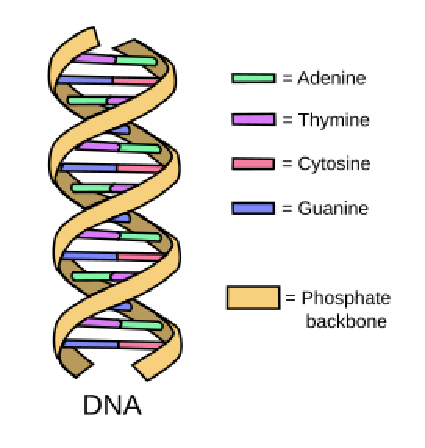
\includegraphics[]{introduction/images/DNA.pdf}
    \caption{Structure and composition of DNA Source: Wikipedia \protect\url{https://en.wikipedia.org/wiki/File:DNA_simple2.svg}}
    \label{intro:fig:dna_rna_pres}
\end{figure}

With mainy complexe and not details her, information contained in DNA is used to build essential molecules that keep the organism alive, reproduce it. This information is therefore the basis of the organism's functioning. If this information is destroyed or modified, the living organism will behave differently or die. So, knowing and understanding the succession of DNA bases is therefore (but not the only one) an effective entry point for analyzing many biological phenomena, disease, evolution,…

To read this information, we have many biochemical techniques that we group under the term Sequencing techniques. There technics will allow us to read fractions of DNA fragments more or less long and with a variable error rate.

\section{Sequencing} \label{section:introduction:sequencing}

Sequencing technology evolve quickly since 1977\cite{sanger_sequencing}, even if it is an a posteriori reconstruction, three generations can be distinguished, based on reads property. In this section we didn't detail the biochemical methods we just focus on reads property and her impact on different bioinformatics task.

The two most important properties of a read are its size and error rate. The longer of a read provide more information about his original sequence, which facilitate downstream analysis. If read contains many errors (replace a letter by an other one, insert random data or skip a part of data), the cost of downstream analysis increase and lost in precision and recall.

\begin{table}[ht]
    \centering
    \begin{tabular}{ll|rr|l}
Generation & Technology          & Read length (bd)                 & Error rate             & Source                          \\ \hline
Second     & ABI/Solid           & 75                               & Low ($\approx$ 2\%)    & \cite{seq_assembly_demystified} \\
Second     & Illumina/Solexa     & 100–150                          & Low (<2\%)             & \cite{seq_assembly_demystified} \\
Second     & IonTorrent          & $\approx$ 200                    & Medium ($\approx$ 4\%) & \cite{seq_assembly_demystified} \\
Second     & Roche/454           & 400–600                          & Medium ($\approx$ 4\%) & \cite{seq_assembly_demystified} \\
First      & Sanger              & $\approx$ 2 kb                   & Low ($\approx$ 2\%)    & \cite{seq_assembly_demystified} \\
Third      & Pacific Biosciences & $\approx$ 10 kb ($\max$ 100 kb)  & High ($\approx$ 18\%)  & \cite{seq_assembly_demystified} \cite{longread_dark_matter} \\
Third      & Oxford Nanopore     & $\approx$ 10 kb ($\max$ 1 mb)    & High ($\approx$ 12\%)  & \cite{longread_dark_matter} \cite{nanopore_read_accuracy} \\
    \end{tabular}
    \caption{This table present length of reads and error rate of main sequencing technology. Pacific Biosciences and Oxford Nanopore evolve quickly and this value change we have tried to be as up-to-date as possible but between two publications these values vary considerably.}
    \label{intro:tab:technology_property}
\end{table}

Sanger technique create large reads with very small error rate, but with a very low throughput and very expensive cost per base.
Second generation increase the throughput and reduce the cost per base, by reducing the length of the reads and increasing the probability of error ($\approx$ 1\%). This type of error are most of the time a substitution between two nucleotides, sequencer read \texttt{A} in place of a \texttt{T}.
The third generation has greatly increased the size of the reads but also the error rate while maintaining a descent throughput. Error in third generation are mostly insertion deletion, sequencer didn't read a part of sequence or generate random base not present in original sequence. Table \ref{intro:tab:technology_property} present read length and error rate on many sequencing technology.

DNA sequencing was very useful tools for many analysis, and in some cases is mandatory to be able to understand biological mechanisms. 

With sequencing we can read all information contains in genome, but we have only some small unordered fragment, the genome assembly designate the task of reconstruct the original sequence from this small unordered fragment.

\section{Algorithms for genome assembly}

If you want study an organism, knowing the complete genome sequence is very useful for a lot of task like find the genes or the sequence variations across a population, understand how speciation affect genome. Yet, the best sequencing technologies still provide reads that are at least 2 orders of magnitude shorter than the genome. To understand the assembly problem, we provide a useful analogy which, to the best of our knowledge, has never been formulated before.

Imagine a crazy copyist monk. He is copying a book but he randomly chooses where he starts to copy, and he only copies small fragments of text at a time.
The copyist monks make errors, e.g. he would sometimes replaces a symbol by another one, would skip a symbol, or would add a random symbol. We respectively call these errors substitutions, deletions and insertions.
Now imagine that there are multiple such copyist monks.
They choose randomly where they begin to write. They can choose several times the same region of the book, never choose to copy a certain region, or more rarely copy another region. We refer by "coverage" the number of times a given chunk of the original book is copied. Coverage may significantly differ from one region to another.
In this analogy, the book is the genome of the organism we want to study, and the copyist monks are our sequencer. The fragments of text are reads, and the operation to rebuild the book is assembly.

The assembly task can be summary has a ordering problem we try to put the text fragments in the original book order, and merge common part at the end.

To carry out this ordering, we can randombly take a fragment of text and search among all the others which begins by the end of the our fragment, the prefix of the second fragment corresponds to the suffix of the first fragment. When we observe this phenomenon we say that the two fragments overlap. Once we have found the best overlap (generaly the longest) for a text fragment we can fuse the two fragments into one and restart our search for a new fragment that overlaps with the one we just created. And so on until we're no more fragments. This definition of the task of assembly is very simple and we will see in more detail some assembly algorithm details in chapter \ref{chapter:sota}.

\section{Assembly glossary} 

Assembly community like any other scientific community create her own slang, to designate object they manipulate.

A \textbf{reads} designate a fragment of DNA produced by sequencer and when to read share a common part at their end they share an \textbf{overlap}, the length of this common part was the length of overlap.

A \textbf{contig} designates a sequence of DNA produced by an assembly tools. Exact definition of what is a \textbf{contig} changes between each assembly tool. We can see in some publication the term \textbf{unitig}. The only thing common in \textbf{unitig} definition was \textbf{contig} was builded from \textbf{unitig}.

A \textbf{scaffold} designates an ordering of contigs many times we can't reconstruct each chromosome in one contig. We describe some reasons of this fragmentation later. But with external informations, restriction card, linked read, target sequencing, we can order contigs and determinate approximately the number of bases between each of them and become near to the real genome easily.

\section{Thesis outline}

Chapter \ref{chapter:preassembly} presents the work that was done on the steps before assembly. The quality of the data that is provided to the assemblers has a direct impact on the result that will be produced. This chapter contains a blog post about the state of the art of tools they search overlap between DNA fragment and how to compare this tools. The rest of the chapter is a paper that present two tools, \yacrd that will detect and remove regions with very high error rates in reads, without this low quality region assembly tools perform a better work. And \fpa which will allow to filter the common region found between the reads which are interesting.

Chapter \ref{chapter:sota} presents a state of the art of the different assembly methods, both from a theoretical point of view and by presenting how the tools work in practice.

Chapter \ref{chapter:postassembly} contains a blog post that presents the difficulties of evaluating assembly tools that do not correct reads or even contigs. As well chapter \ref{chapter:postassembly} present our tool for analyzing and improving assembly results, \knot that we developed during this thesis.

Chapter \ref{chapter:other_contribution} will focus on my scientific contributions that have not been important enough to have a dedicated chapter. Participation in the development of a graphical interface for genomic data analysis. My participation in the CAMI2 contest. And some work around 10X data.

%\onlyinsubfile{
%\bibliographystyle{plainnat}
%\bibliography{main}
%\addcontentsline{toc}{chapter}{Bibliography}
%}

\end{document}